\documentclass[11pt,letterpaper,titlepage]{scrartcl}
\usepackage[utf8]{inputenc}
\usepackage{amsmath}
\usepackage{mathtools}
\usepackage{amsfonts}
\usepackage{amssymb}
\usepackage{enumerate}
\usepackage{graphicx}
\usepackage{tikz}
\usetikzlibrary {positioning}
\usepackage{color}
\usepackage{algorithm}
\usepackage[noend]{algpseudocode}
\renewcommand\textproc{}
\usepackage{pgfplots}
\setlength{\parindent}{0pt}
\setlength{\parskip}{1em}
\usepackage{listings}
\usepackage[headings]{fullpage}
\usepackage{multirow}
\usepackage[paper=a4paper,margin=2cm]{geometry}
\pgfplotsset{compat=1.15}

% Customizing
\definecolor{mygreen}{rgb}{0,0.6,0}
\definecolor{mymauve}{rgb}{0.58,0,0.0}
\lstset{ %
  basicstyle=\ttfamily,
  keepspaces=true,
  tabsize=2,
  commentstyle=\color{mygreen},
  language=Python,
  keywordstyle=\color{mymauve}
}
\definecolor{nodeColor}{RGB}{230,230,230}
\definecolor{forward}{RGB}{200,15,15}
\definecolor{backward}{RGB}{60,150,210}
\definecolor{quer}{RGB}{60,180,0}

% Commands
\newcommand{\bigO}{\mathcal{O}}
\newcommand{\Epsilon}{\mathcal{E}}
\newcommand{\EV}{\mathbb{E}}
\newcommand{\Var}{\mathrm{Var}}
\newcommand{\Bin}[1]{\mathrm{Bin}{\left({#1}\right)}}
\newcommand{\Poi}[1]{\mathrm{Poi}{\left({#1}\right)}}
\newcommand{\Geo}[1]{\mathrm{Geo}{\left({#1}\right)}}
\newcommand{\qed}[1]{{\:}_\square}
\newcommand{\eqtext}[1]{\ensuremath{\stackrel{\text{#1}}{=}}}

% Meta
\newcommand{\name}{Daniel Sparber}
\newcommand{\course}{CIS 677}
\newcommand{\taskName}{Homework 4}

% Header & Footer
\usepackage{fancyhdr}
\pagestyle{fancy}
\fancyhf{}
\rhead{\name}
\chead{\course}
\lhead{\taskName}
\cfoot{Page \thepage}

\fancypagestyle{firstpage}{
  \fancyhead{}
  \cfoot{Page \thepage}
}

\begin{document}

\title{\course - \taskName}
\author{\name}
\date{\today}

\newgeometry{left=2cm,right=2cm,bottom=3cm, top=3cm}


\thispagestyle{firstpage}

\course \vspace{5pt} 
\\ {\LARGE{\textbf{\taskName}}} \vspace{5pt} 
\\ {\Large \name}

\rule{\textwidth}{0.4pt}

\section*{Problem 1}

\subsection*{Input}

Matrix $M \in \mathbb{R}^{n \times n}$

\subsection*{Output}

Return \texttt{true} if $M$ is a diagonal matrix, \texttt{false} otherwise.

\subsection*{Algorithm}

\underline{Algorithm A}

\begin{enumerate}
    \item Pick $v \in \{0,1\}^n$ uniformly at random.
    \item Calculate $x = Mv$
    \item Calculate $y = Mu$, where $u = [1,\cdots,1]^T$
    \item Return \texttt{true} if $\forall i \in \{1,\dots,n\}: y_i \cdot v_i = x_i$, otherwise \texttt{false}
\end{enumerate}

\underline{Algorithm B}

Repeat Algorithm A $\operatorname{log} n$ times. If A always outputs \texttt{true}, return \texttt{true}, otherwise return \texttt{false}.

\subsection*{Analysis}

\subsubsection*{Runtime}

Algorithm A performs exactly 2 matrix-vector query. Algorithm B calls A $\operatorname{log} n$ times. Thus, algorithm B queries $\bigO(\operatorname{log} n)$ vector-matrix products.

\subsubsection*{Correctness}

Let $M  \in \mathbb{R}^{n \times n}$ be arbitrary.

\textbf{Case 1:} $M$ is diagonal

\underline{Claim} 

Algorithm B accepts

\underline{Proof}

\textit{Lemma 1:} Given $M$ is diagonal, algorithm A always returns \texttt{true}.

Let $v \in \{0,1\}^n$ be arbitrary, $M$ is diagonal.

$d_i$, $i \in \{1,\dots,n\}$ denotes the $i$-th diagonal element of $M$.

$x = Mv = [d_1 v_1,\dots, d_n v_n]^T$

$y = Mu = [d_1,\dots,d_n]^T$

$\forall i \in \{1,\dots,n\}$: $y_i \cdot v_i = d_i \cdot v_i = x_i$. Thus, the algorithm A returns \texttt{True}.

\textit{Using lemma 1:}

A always returns \texttt{true}. Thus, B returns \texttt{true}.

\textbf{Case 2:} $M$ is not diagonal

\underline{Claim} 

Algorithm B rejects with probability at least $1 - \frac{1}{n}$, i.e. $\operatorname{Pr}[\textit{B error}] \leq \frac{1}{n}$

\underline{Proof}

\textit{Lemma 2:} Given M is not diagonal, algorithm A rejects with probability at least $\frac{1}{2}$, i.e. $\operatorname{Pr}[\textit{A error}] \leq \frac{1}{2}$

Let $v \in \{0,1\}^n$ be arbitrary, $M$ is not diagonal.

Since $M$ is not diagonal, $m_{i,j} \neq 0$ for some, $i,j \in \{1,\dots,n\}$ where $i \neq j$

$\operatorname{Pr}[\textit{A error}] \leq
\operatorname{Pr}][\textit{Error in line i}] =
\operatorname{Pr}[y_i \cdot v_i = x_i] = 
\operatorname{Pr}[y_i \cdot v_i - x_i = 0]$

$x_i = m_{i,j} \cdot v_j + \sum_{k \in \{1,\cdots,n\} k \neq j} m_{i,k}\cdot v_k$

$y_i \cdot v_i = m_{i,j} \cdot v_i + \sum_{k \in \{1,\cdots,n\} k \neq j} m_{i,k}\cdot v_i$

$y_i\cdot v_i - x_i =  m_{i,j} \cdot v_i - m_{i,j} \cdot v_j + S$, where $S = \sum_{k \in \{1,\cdots,n\} k \neq j} m_{i,k}\cdot (v_i - v_k)$

\begin{itemize}
    \item Case $S = 0$:

    $\operatorname{Pr}[\textit{A error}] \leq  
    \operatorname{Pr}[m_{i,j} \cdot v_i - m_{i,j} \cdot v_j = 0] =
    \operatorname{Pr}[v_i = v_j] =
    \frac{1}{2}$

    \item Case $S \neq 0$:

    $\operatorname{Pr}[\textit{A error}] \leq  
    \operatorname{Pr}[m_{i,j} \cdot v_i - m_{i,j} \cdot v_j + S = 0] \leq
    \operatorname{Pr}[v_i \neq v_j] =
    \frac{1}{2}$
    
\end{itemize}




\textit{Using lemma 2:}

$\operatorname{Pr}[\textit{B error}] =
(\operatorname{Pr}[\textit{A error}])^{\operatorname{log} n} \leq \frac{1}{2}^{\operatorname{log} n} = 
\frac{1}{n}$ 

\pagebreak
\section*{Problem 2}

\subsection*{Claim}

C = BPP


\subsection*{Proof}

By proofing C $\subseteq$ BPP and BPP $\subseteq$ C.

\subsubsection*{BPP $\subseteq$ C}

Let $L \in$ BPP be arbitrary.

By definition of BPP: There exists a poly-time algorithm A which on any input $x$ has the following behavior:

\begin{itemize}
    \item If $x \in L$, then $\operatorname{Pr}[\textit{A accepts } x] > \frac{3}{4}$
    
    \item If $x \notin L$, then $\operatorname{Pr}[\textit{A rejects } x] > \frac{3}{4}$
\end{itemize}

A is also a valid algorithm for C, since A fulfills the definition of C:

Let $\operatorname{poly}(n) = 4$:

\begin{itemize}
    \item If $x \in L$, then $\operatorname{Pr}[\textit{A accepts } x] \geq \frac{3}{4} = \frac{1}{2} + \frac{1}{4} = \frac{1}{2} + \frac{1}{\operatorname{poly}(n)}$
    
    \item If $x \notin L$, then $\operatorname{Pr}[\textit{A rejects } x] \geq \frac{3}{4} \geq \frac{1}{2}$
\end{itemize}

\subsubsection*{C $\subseteq$ BPP}

Let $L \in$ C be arbitrary.

By definition of C: There exists a poly-time algorithm A which on any input $x$ has the following behavior:

\begin{itemize}
    \item If $x \in L$, then $\operatorname{Pr}[\textit{A accepts } x] \geq \frac{1}{2} + \frac{1}{\operatorname{poly}(n)}$
    
    \item If $x \notin L$, then $\operatorname{Pr}[\textit{A rejects } x] \geq \frac{1}{2}$
\end{itemize}

Let B be an algorithm defined as follows:

\begin{itemize}
    \item Repeat algorithm A $k$ times. Accept, if at least $l = \frac{k}{2} + \frac{k}{2 \operatorname{poly}(n)}$ of executions of A accepted, otherwise reject.
\end{itemize}

Where $k = 32(\operatorname{poly}(n))^2\operatorname{log}(2)$

\underline{Claim}

B is a valid algorithm for BPP, i.e. B has the following properties:

\begin{itemize}
    \item If $x \in L$, then $\operatorname{Pr}[\textit{B accepts } x] > \frac{3}{4}$
    
    \item If $x \notin L$, then $\operatorname{Pr}[\textit{B rejects } x] > \frac{3}{4}$
\end{itemize}

\underline{Proof}

\begin{itemize}
    \item Assume $x \in L$:

Let $X_i$ be a 0/1 random variable, that indicates if the $i$-th execution of A accepted.

Let $X = \sum\limits_{i=1}^k X_i$,
$E[X] = k \cdot \left( \frac{1}{2} + \frac{1}{\operatorname{poly}(n)} \right) = \frac{k}{2} + \frac{k}{\operatorname{poly}(n)}$

$\operatorname{Pr}[\textit{B accepts } x] 
= \operatorname{Pr}[\textit{A accepts } x \textit{ at least l times}]
= \operatorname{Pr}[X \geq l] 
= 1 - \operatorname{Pr}[X < l]
= 1 - \operatorname{Pr}[X \leq l]$

$X$ consists of independent 0/1 random variables, thus Chernoff bounds with additive error can be applied:

$\operatorname{Pr}[X \leq l]= \operatorname{Pr}\left[X \leq  \frac{k}{2} + \frac{k}{2 \operatorname{poly}(n)}\right]
= \operatorname{Pr}\left[X \leq  \left(\frac{k}{2} + \frac{k}{\operatorname{poly}(n)}\right) - k\cdot\frac{1}{2\operatorname{poly}(n)}\right]
< e^{-\frac{\frac{1}{(2\operatorname{poly}(n))^2} k}{2}}
$

$=
e^{-\frac{\frac{1}{4 (\operatorname{poly}(n))^2} 32(\operatorname{poly}(n))^2\operatorname{log}(2)}{2}} 
=
e^{-\operatorname{log}(16)}
= \frac{1}{16} \leq \frac{1}{4}$

$\Rightarrow
\operatorname{Pr}[\textit{B accepts } x] > \frac{3}{4}$ 

\item Assume $x \notin L$:

Let $Y_i$ be a 0/1 random variable, that indicates if the $i$-th execution of A accepts.

Let $Y = \sum\limits_{i=1}^k Y_i$,
$E[Y] = k \cdot\frac{1}{2} = \frac{k}{2}$

$\operatorname{Pr}[\textit{B rejects } x] 
= \operatorname{Pr}[\textit{A accepts } x \textit{ less than l times}]
= \operatorname{Pr}[Y < l] 
= 1 - \operatorname{Pr}[Y \geq l]$

Applying Chernoff:

$\operatorname{Pr}[Y \geq l]
= \operatorname{Pr}\left[Y \geq \frac{k}{2} + \frac{k}{2 \operatorname{poly}(n)}\right]
= \operatorname{Pr}\left[Y \geq \frac{k}{2} + k\cdot\frac{1}{2\operatorname{poly}(n)}\right]
< e^{-\frac{\frac{1}{(2\operatorname{poly}(n))^2} k}{4}}$

$=
e^{-\frac{\frac{1}{4(\operatorname{poly}(n))^2} 32(\operatorname{poly}(n))^2\operatorname{log}(2)}{4}} 
=
e^{-\operatorname{log}(4)}
= \frac{1}{4}$

$\Rightarrow
\operatorname{Pr}[\textit{B rejects } x] > \frac{3}{4}$ 

\end{itemize}

Since A is a polynomial-time algorithm and A is executed $32(\operatorname{poly}(n))^2\operatorname{log}(2)$ times, B is a polynomial-time algorithm.

Thus, B is a valid algorithm for BPP.

\pagebreak


\section*{Problem 3}

First consider the case, where all colors are available for a given node $v$. Since $\Delta$ is the maximum degree in $G$, $v$ has at most $\Delta$ neighbors. In the worst case, those $\Delta$ neighbors all need to be colored with different colors. Even so, there are still $2 \Delta - \Delta = \Delta$  colors remaining to color $v$. Thus, there are at least $\Delta$ good colors for $v$.

For every node $2 \log n$ colors are picked uniformly at random. The following steps calculate a lower bound for the probability of picking at least one good color for every node. 

Let $v \in V$ be arbitrary.

$\Pr[\textit{Picking a good color for v with one trial}] \geq \frac{\Delta}{2\Delta} = \frac{1}{2}$

$\Rightarrow \Pr[\textit{Picking a bad color for v with one trial}] \leq \frac{1}{2}$

$\Rightarrow \Pr[\textit{Picking only bad colors for v (with } 2\log n \textit{ trials)}] \leq 
\left(\frac{1}{2}\right)^{2 \log n} = 
2^{-2 \log n} = 
n^{-2} = 
\frac{1}{n^2}$

$\Rightarrow \Pr[\textit{Some node picks only bad colors}] \leq n \cdot \frac{1}{n^2} = \frac{1}{n}$

$\Rightarrow \Pr[\textit{All nodes pick at least one good color}] = 
1 - \Pr[\textit{Some node picks only bad colors}] \geq 1 - \frac{1}{n}$

Therefore, the probability that a $(2\Delta)$-coloring of the graph, such that every vertex is assigned only one of the colors it has sampled, exists with propability at least $1 - 1/n$.

\pagebreak
\section*{Problem 4}

Let $U = \{1,2,\dots,n\}$

For any integer $x$, $x_k$ is the $k$-th bit of $x$ in binary representations

\subsection*{Part a - Deterministic algorithm}

Let $U = \{1,2,\dots,n\}$

For any integer $x$, $x_k$ is the $k$-th bit of $x$ in binary representations

\subsubsection*{Input}

$V \in \mathbb{R}_{_{\geq 0}}^n$, with at least one non-zero element.

\subsubsection*{Output}

Returns unique index $i$ such that $V[i] \neq 0$ whenever $V$ contains exactly one non-zero element. Otherwise outputs ``More than one non-zero entry''.

\subsubsection*{Algorithm}


\begin{enumerate}
    \item $a = 0$

    \item For $k \in \{0,\dots, \lceil \log n \rceil\}$:

    \begin{itemize}
        \item $S_k := \{s ~ | ~ s \in U \text{ if } s_k = 0 \}$
                
        \item if $Q(S_k) \neq 0$ and $Q(U \setminus S_k) \neq 0$: return ``More than one non-zero entry''
        
        \item $a_k = 1$ if $Q(S_k) \neq 0$ else $0$
        
    \end{itemize}
    
    \item return $a$
\end{enumerate}


\subsubsection*{Run time}

Run time in terms of summation queries:

Every iteration performs $\bigO(1)$ queries. There is a total number of $\lceil \log n \rceil$ iterations.

Thus, the algorithm performs $\bigO(\log n)$ summation queries.

\subsubsection*{Correctness}

\begin{itemize}
    \item Case 1: More than one non-zero entry
    
    There exists $i, j \in U$ with $i \neq j$, $V[i] > 0$ and $V[j] > 0$.
    
    Since $i \neq j$, there exists at least one index $k$ with $i_k \neq j_k$.
    
    Thus, only $i$ or $j$ is in $S_k$. Therefore, $Q(S_k) > 0$ and $Q(U \setminus S_k) > 0$
    
    The algorithm always outputs ``More than one non-zero entry''

    
    \item Case 2: Exactly on non-zero entry
    
    There exists a unique $b$ with $V[b] > 0$
    
    For every $k \in \{0,\dots, \lceil \log n \rceil\}$:
    
    \begin{itemize}
        \item Case $b_k = 0$: $b \notin S_k$, since $V[b]$ is the only non-zero element: $Q(S_k) = 0 \Rightarrow a_k = 0$
    
        \item Case $b_k = 1$: $b \in S_k \Rightarrow Q(S_k) = V[b] > 0 \Rightarrow a_k = 1$,
        
        \item Therefore $b_k = a_k$

    \end{itemize}
    
    $\Rightarrow a = b$
    
    Since $b$ is unique, the algorithm returns the only correct index.
    
\end{itemize}

\pagebreak

\subsection*{Part b - Randomized algorithm}

\subsubsection*{Input}

$V \in \mathbb{R}_{_{\geq 0}}^n$, with exactly $d \in [1..n]$ non-zero elements, accuracy parameter $\delta$.

\subsubsection*{Output}

Returns an index $i$ with $V[i] \neq 0$ with probability of at least $1 - \delta$.

\subsubsection*{Algorithm}

\begin{itemize}
    \item Repeat $k$ times:
    \begin{enumerate}
        \item For $i \in [1..n]$: Draw $x_i \in \{0, 1\}$ with $\Pr[x_i = 1] = \frac{1}{d}$ 
        
        \item Let $S = \{i ~| ~ i \in [1..n] \text{ if } x_i = 1\}$
        
        \item If $Q(S) \neq 0$:
                
        \begin{itemize}
            \item Run deterministic algorithm with the following modification:
            
            Instead of using $S_k$, $S_k^\prime = \{s ~ | ~ s \in S_k \text{ if } x_s = 1\}$ is used.
            
            Instead of using $\Bar{S_k}$, $\Bar{S_k}^\prime = \{s ~ | ~ s \in \Bar{S_k} \text{ if } x_s = 1\}$ is used.
            
            \item If index is returned by deterministic algorithm: return index
            
        \end{itemize}
        
    \end{enumerate} 
    
    \item return $0$
\end{itemize} 

Where $k = 9 \cdot \log(1/\delta)$ and $Q_W(S) = \sum_{j \in S} W[j]$ is the summation query over vector $W$

\subsubsection*{Run time}

If $d = 1$, the algorithm runs in $\bigO(\log n)$.

Otherwise, one iteration of the algorithm performs one summation query plus at most $\bigO(\log n)$ summation queries by calling the deterministic algorithm.

Thus, one iteration performs $\bigO(\log n)$ summation queries.

By repeating $k \in \bigO(\log(1/\delta))$ times, the total number of summation queries is in  $\bigO(\log(n)\cdot\log(1/\delta))$.

\subsubsection*{Correctness}

\begin{itemize}
    \item Case $d = 1$:
    
    For every $i \in [1,\dots,n]$ $x_i = 1$ with probability $1$. Thus, the algorithm simply performs the deterministic algorithm. One iteration of the randomized algorithm is performed.

    The correctness follows from correctness of deterministic algorithm. The probability of returning the correct index is $1$ and therefore at least $1 - \delta$.
    
    \item Case $d \neq 1$
    
    Every index $i$, where $x_i = 0$, is never in any set $S_k^\prime$ and $\Bar{S_k}^\prime$. Thus, both summation queries never contains $V[i]$. 
    
    Likewise, every index $i$, where $x_i = 1$ is always in $S_k^\prime$ whenever $i$ is in $S_k$ and in $\Bar{S_k}^\prime$ whenever $i$ is in $\Bar{S_k}$
    
    Let $W = [V[0]\cdot x_0,\dots,V[n]\cdot x_n]$
    
    For this definition of $W$, performing the summation queries on $W$ with $S_k$ and $\Bar{S_k}$ is equivalent to performing the summation query on $V$ with $S_k^\prime$ and $\Bar{S_k}^\prime$. In the following steps, the equivalent problem, using $W$ is analyzed.
    
    
    \underline{Analyzing one iteration:}
    
    \textit{Claim:} $W$ contains exactly one non-zero element with probability $p \geq \frac{1}{4}$
    
    \textit{Proof:} 
    
    Every index with a zero element in $V$ is also an index with a zero element in $W$ by construction of $W$.
    
    Therefore, only non-zero elements of $V$ might remain in $W$. By construction, each of the $d$ non-zero element remains in $W$ with probability $\frac{1}{d}$. Let $X$ be the amount of non-zero elements remaining in $W$.
    
    $X \sim \operatorname{Binomial}\left(d, \frac{1}{d}\right)$
    
    $\Pr[X = 1] = 
    {d \choose 1} \cdot \frac{1}{d} \cdot \left(1 - \frac{1}{d}\right)^{d-1} = 
    \left(1 - \frac{1}{d}\right)^{d-1} =
    \frac{\left(1 - \frac{1}{d}\right)^{d} }{1 - \frac{1}{d}} \geq
    \frac{\left(1 - \frac{1}{d}\right)^{d} }{1 - 0} = 
    \left(1 - \frac{1}{d}\right)^{d} 
    $ 
    
    Since $d \in [1..n]$ and $d \neq 1$: $d \geq 2$ 

    For $d = 2$: $\left(1 - \frac{1}{d}\right)^{d} = \frac{1}{4}$
        
    The term $\left(1 - \frac{1}{d}\right)^{d}$ is monotonically increasing as $d$ increases (see calculus).  
    
    Thus, $\left(1 - \frac{1}{d}\right)^{d} \geq \frac{1}{4}$
    
    $\Rightarrow \Pr[X = 1] \geq \frac{1}{4}$
    
    \textit{q.e.d}
    
    The if condition ensures, that $W$ contains at least one non-zero element.
    
    Therefore, the input conditions for the deterministic algorithm are met. 
    
    Whenever $W$ contains exactly one non-zero element, the correct index of that element is returned by the deterministic algorithm. Otherwise, a string is returned.
    
    By construction of $W$, this index is also a valid non-zero index in the original vector. Hence, the entire algorithm succeeds and returns a valid index.
    
    The probability of $W$ containing exactly one non-zero element is $p \geq \frac{1}{4}$. Thus, one iteration succeeds with $p \geq \frac{1}{4}$.
    
    \underline{After $k$ iterations}
    
    The algorithm returns a correct element whenever one iteration returns.
    
    The algorithm can only fail, if no valid index was found within $k$ iterations, i.e. if every iteration fails.
    
    $\Rightarrow \Pr[\textit{error}] \leq 
    (1 - p)^k \leq 
    \left(1 - \frac{1}{4}\right)^k = 
    \left(\frac{3}{4}\right)^k = 
    e^{k \cdot \log(3/4)} = $
    
    $ = e^{9 \cdot \log(1/\delta) \cdot \log(3/4)} \leq
    e^{\frac{- 1}{\log(3/4)} \cdot \log(1/\delta) \cdot \log(3/4)} = 
    e^{-\log(1/\delta)} = 
    e^{\log \delta} =
    \delta$
    
    $\Rightarrow \Pr[\textit{success}] = 1 - \Pr[\textit{error}] \geq 1 - \delta$
    
\end{itemize}



\pagebreak
\section*{Problem 5}

Consider the following directed graph for $n \geq 3$:

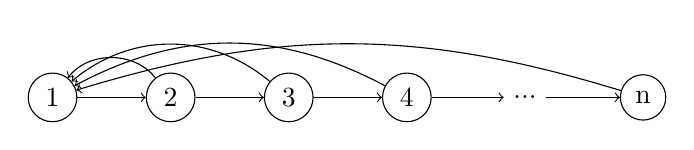
\begin{tikzpicture}
    \node[shape=circle,draw=black] (1) at (0,0) {1};
    \node[shape=circle,draw=black] (2) at (1.5,0) {2};
    \node[shape=circle,draw=black] (3) at (3,0) {3};
    \node[shape=circle,draw=black] (4) at (4.5,0) {4};
    \node (i) at (6,0) {...};
    \node[shape=circle,draw=black] (n) at (7.5,0) {n} ;

    \path [->](1) edge node [left] {}(2);
    \path [->](2) edge node [left] {}(3);
    \path [->](3) edge node [left] {}(4);
    \path [->](4) edge node [left] {}(i);
    \path [->](i) edge node [left] {}(n);
    
    \path [->](2) edge [bend right=52] node [right] {}(1);
    \path [->](3) edge [bend right=40] node [right] {}(1);
    \path [->](4) edge [bend right=28] node [right] {}(1);
    \path [->](n) edge [bend right=17] node [right] {}(1);

\end{tikzpicture}

This graph has a the directed edges $(i, i+1)$ and $(i+1, 1)$ for $1 \leq i < n$.

Thus, the graph has the a transition matrix $P \in [0, 1]^{n \times n}$ with the following entries:

$p_{1,2} = 1$,
$p_{n,1} = 1$

For $2 \leq i < n$: $p_{i, i + 1} = 0.5$ and $p_{i, 1} = 0.5$ 

For all other elements: $p_{i,j} = 0$.

Since the graph is irreducible (strongly connected) and aperiodic (there exits a path of length $n + 2$ and one of length $n + 3$ for every node and $\operatorname{gcd}(n + 2, n + 3) = 1$). Therefore, a unique stationary solution $\pi$ exists . By definition of a stationary solution, the following equation holds:

$\pi = \pi P$

Furthermore, by matrix multiplication we know for $j \in [1..n]$:

$\pi_j = \sum\limits_{i = 1}^n \pi_i \cdot p_{i,j}$

This yields the following linear equations for the given transition matrix $P$:

\begin{enumerate}[I:]
    \item $\pi_1 = \pi_n + 0.5 \cdot \sum\limits_{i = 2}^{n - 1} \pi_i$
    \item $\pi_2 = \pi_1$
    \item For $2 \leq i < n$: $\pi_{i + 1} = 0.5 \cdot \pi_i \Leftrightarrow 2 \cdot \pi_{i + 1} = \pi_{i}$ 
\end{enumerate}

\underline{Claim:} For $n \geq 3$: $2^{n-2}\cdot\pi_n = \pi_2$ 

\underline{Proof:} By induction on $n$, using equation III

Let $n \geq 3$ be arbitrary.

Case $n = 3$: $2^{3-2}\cdot\pi_3 = 2\cdot\pi_3 = \pi_2$

Case $n > 3$: $2^{n-2}\cdot\pi_n = 2^{n-3}\cdot(2 \cdot \pi_n) = 2^{n-3}\cdot(\pi_{n - 1}) = 2^{(n-1)-2}\cdot\pi_{n - 1} = \pi_2$

Therefore, for this graph and $u = 2, v = n$ the following holds:

$\frac{\pi_u}{\pi_v} = \frac{\pi_2}{\pi_n} = \frac{2^{n - 2} \cdot \pi_n}{\pi_n} = 2^{n - 2}$

Thus, $\pi_u/\pi_v = 2^{\Omega(n)}$.

\end{document}
